\documentclass[11pt,class=report,crop=false]{standalone}
\usepackage[screen]{../python}
\begin{document}

% Commande spécifique
\newcommand{\badletter}[1]{\underline{\textcolor{red}{#1}}}



%====================================================================
\chapitre{L-système}
%====================================================================

\objectifs{Les L-systèmes offrent une façon très simple de coder des phénomènes complexes. À partir d'un mot initial et d'opérations de remplacement, on arrive à des mots compliqués. Lorsque l'on \og{}dessine\fg{} ces mots, on obtient de superbes figures fractales. Le \og{}L\fg{} vient du botaniste A. Lindenmayer qui a inventé les L-systèmes afin de modéliser les plantes.
}

\begin{center}
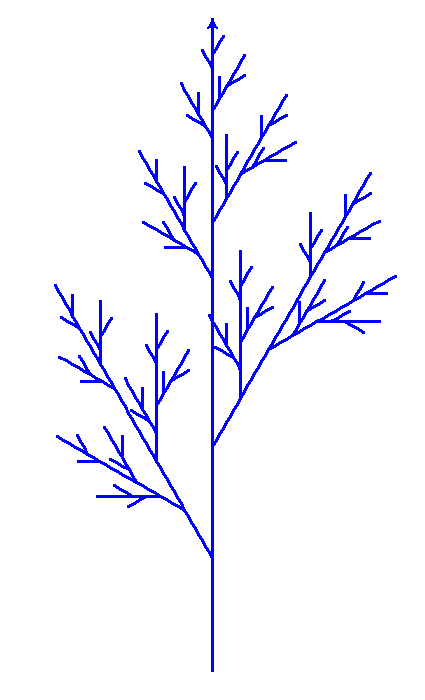
\includegraphics[scale=0.3]{ecran-lsysteme-14}
\end{center}

\index{lsysteme@L-système}
\index{remplacer}
\index{tortue}

%%%%%%%%%%%%%%%%%%%%%%%%%%%%%%%%%%%%%%%%%%%%%%%%%%%%%%%%%%%%%%%%
%%%%%%%%%%%%%%%%%%%%%%%%%%%%%%%%%%%%%%%%%%%%%%%%%%%%%%%%%%%%%%%%

\begin{cours}[L-système]
Un \defi{L-système} est la donnée d'un mot initial et de règles de remplacement.
Voici un exemple avec le mot de départ et une seule règle : \\
\centerline{\mot{BgAdB} \qquad \mot{A} $\rightarrow$ \mot{ABA}}


Le \defi{$k$-ème itéré} du L-système s'obtient en appliquant $k$ fois la substitution au mot de départ.
Avec notre exemple :
\begin{itemize}
  \item Première itération. Le mot de départ est \mot{BgAdB}, la règle est \mot{A} $\rightarrow$ \mot{ABA} : on remplace le \mot{A} par \mot{ABA}. On obtient le mot \mot{BgABAdB}.
  
  \item Deuxième itération. On part du mot obtenu \mot{BgABAdB}, on remplace les deux \mot{A} par \mot{ABA} : on obtient le mot \mot{BgABABABAdB}.
  
  \item Le troisième itéré est \mot{BgABABABABABABABAdB}, etc.  
\end{itemize}

Lorsqu'il y a deux règles (ou plus) il faut les appliquer en même temps.
Voici un exemple de L-système à deux règles :
 \\
\centerline{\mot{A} \qquad \mot{A} $\rightarrow$ \mot{BgA} \qquad \mot{B} $\rightarrow$ \mot{BB}}
Avec notre exemple :
\begin{itemize}
  \item Première itération. Le mot de départ est \mot{A}, on applique la première règle \mot{A} $\rightarrow$ \mot{BgA} (la seconde règle ne s'applique pas, car il n'y a pas encore de \mot{B}): on obtient le mot \mot{BgA}.
  
  \item Deuxième itération. On part du mot obtenu \mot{BgA}, on remplace les \mot{A} par \mot{BgA} et en même temps les \mot{B} par \mot{BB} : on obtient le mot \mot{BBgBgA}.
  
  \item Le troisième itéré est \mot{BBBBgBBgBgA}, etc.  
\end{itemize}

\end{cours}


\begin{cours}[Argument optionnel d'une fonction]

\index{fonction!argument optionnel}
\index{argument}

Je veux programmer une fonction qui trace un trait d'une longueur donnée, avec la possibilité de changer l'épaisseur du trait et la couleur.

Une méthode serait de définir une fonction par : \\
 \centerline{\ci{def tracer(longueur, epaisseur, couleur):}}
 Je l'appellerais alors par exemple par :\\
 \centerline{\ci{tracer(100, 5, "blue"):}} 
Mais comme mes traits auront le plupart du temps l'épaisseur $5$ et la couleur bleue, je perds du temps et de la lisibilité en redonnant ces informations à chaque fois.

\medskip

Avec \Python{} il est possible de donner des arguments optionnels. Voici une meilleure façon de faire en donnant des valeurs par défaut :\\
 \centerline{\ci{def tracer(longueur, epaisseur=5, couleur="blue"):}}
 
\begin{itemize}
  \item La commande \ci{tracer(100)} trace mon trait, et comme je n'ai précisé que la longueur, les arguments \ci{epaisseur} et \ci{couleur} prennent les valeurs par défaut ($5$ et bleu).
  
   \item La commande \ci{tracer(100, epaisseur=10)} trace mon trait avec une nouvelle épaisseur (la couleur est celle par défaut).
   
    \item La commande \ci{tracer(100, couleur="red")} trace mon trait avec une nouvelle couleur (l'épaisseur est celle par défaut).  
    
     \item La commande \ci{tracer(100, epaisseur=10, couleur="red")} trace mon trait avec une nouvelle épaisseur et une nouvelle couleur.
     
     \item Voici aussi ce que tu peux utiliser :
     \begin{itemize}
       \item \ci{tracer(100, 10, "red")} : ne pas préciser les noms des options si on fait attention à l'ordre.
       \item \ci{tracer(couleur="red", epaisseur=10, longueur=100)} : on peut nommer n'importe quelle variable, les variables nommées peuvent passer en argument dans n'importe quel ordre !
 
  \end{itemize}   
\end{itemize}   
\end{cours}



%%%%%%%%%%%%%%%%%%%%%%%%%%%%%%%%%%%%%%%%%%%%%%%%%%%%%%%%%%%%%%%%
% Activité 1 - 
%%%%%%%%%%%%%%%%%%%%%%%%%%%%%%%%%%%%%%%%%%%%%%%%%%%%%%%%%%%%%%%%

\begin{activite}[Tracer un mot]

\objectifs{Objectifs : tracer un dessin à partir d'un \og{}mot\fg{}. Chaque caractère correspond à une instruction de la tortue.}

On te donne un mot (par exemple \mot{AgAdAAdAdA}) dans lequel chaque lettre (lues de gauche à droite) correspond à une instruction pour la tortue \Python{}.

\begin{itemize}
  \item \mot{A} ou \mot{B} : avance d'une quantité fixée (en traçant),
  \item \mot{g} : tourne à gauche, sans avancer, d'un angle fixé (le plus souvent $90$ degrés),
  \item \mot{d} : tourne à droite d'un angle fixé.
\end{itemize}

Les autres caractères ne font rien. (On ajoutera d'autres commandes plus loin).

Programme une fonction \ci{trace_lsysteme(mot,angle=90,echelle=1)}
qui affiche le dessin correspondant aux lettres de \ci{mot}. Par défaut l'angle est de $90$ degrés, et à chaque fois que l'on avance, c'est de $100 \times$\ci{echelle}.

Par exemple : \ci{trace_lsysteme("AgAdAAdAdA")} affiche ceci :
\begin{center}
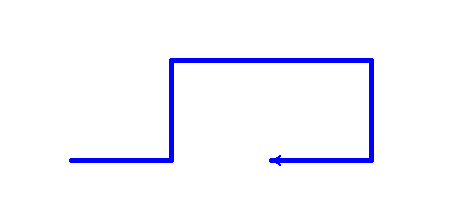
\includegraphics[scale=0.6]{ecran-lsysteme-1}
\end{center}

\end{activite}


%%%%%%%%%%%%%%%%%%%%%%%%%%%%%%%%%%%%%%%%%%%%%%%%%%%%%%%%%%%%%%%%
% Activité 2
%%%%%%%%%%%%%%%%%%%%%%%%%%%%%%%%%%%%%%%%%%%%%%%%%%%%%%%%%%%%%%%%

\begin{activite}[Une seule règle -- Flocon de Koch]

\index{flocon de Koch}

\objectifs{Objectifs : tracer le flocon de Koch à partir d'un mot obtenu par itérations.}

\begin{center}
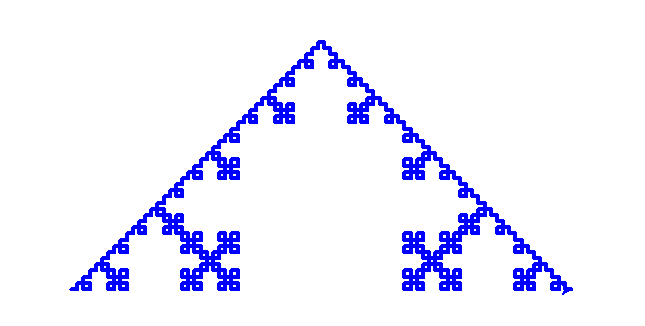
\includegraphics[scale=0.4]{ecran-lsysteme-2}
\end{center}

\begin{enumerate}
  \item Programme une fonction \ci{remplacer_1(mot,lettre,motif)} qui remplace une lettre par un motif dans un mot. 

Par exemple avec \ci{mot = "AdAAg"}, \ci{remplacer_1(mot,"A","Ag")} renvoie le mot \ci{AgdAgAgg} : chaque lettre \mot{A} a été remplacée par le motif \mot{Ag}.
 
  \item Programme une fonction \ci{iterer_lsysteme_1(depart,regle,k)}
  qui calcule le $k$-ème itéré du L-système associé au mot initial \ci{depart} selon la règle \ci{regle} qui contient le couple formé de la lettre et de son motif de remplacement.
  Par exemple, avec :
  \begin{itemize}
    \item \ci{depart = "A"}
    \item \ci{regle = ("A","AgAdAdAgA")} c'est-à-dire \mot{A} $\rightarrow$ \mot{AgAdAdAgA}
    \item pour \ci{k = 0}, la fonction renvoie le mot de départ \ci{A},
    \item pour \ci{k = 1}, la fonction renvoie \ci{AgAdAdAgA},
    \item pour \ci{k = 2}, la fonction renvoie :\\ \centerline{\ci{AgAdAdAgAgAgAdAdAgAdAgAdAdAgAdAgAdAdAgAgAgAdAdAgA}}
    \item pour \ci{k = 3}, la fonction renvoie : \ci{AgAdAdAgAgA...} un mot de $249$ lettres.
    
  \end{itemize}
  
  \item Trace les premières images du  flocon de Koch donné comme ci-dessus par : \\
  \centerline{départ : \mot{A} \qquad règle : \mot{A} $\rightarrow$ \mot{AgAdAdAgA}} 
  
  
  Ici les images pour $k=1$ jusqu'à $k=5$.
  Pour $k=1$, le mot est \mot{AgAdAdAgA} et tu peux vérifier le tracé sur la première image.
  
\begin{center}
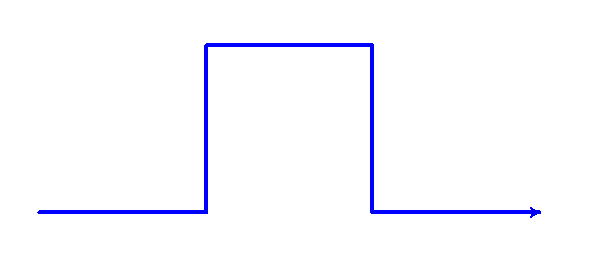
\includegraphics[scale=0.22]{ecran-lsysteme-3a}
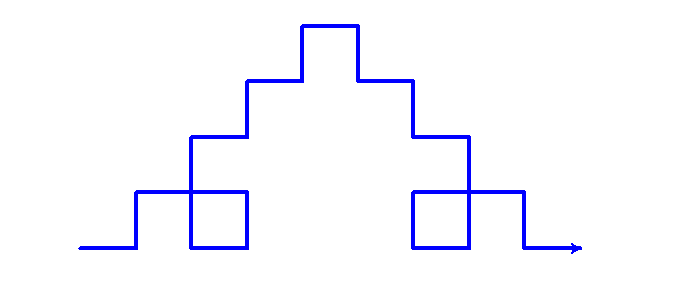
\includegraphics[scale=0.22]{ecran-lsysteme-3b}
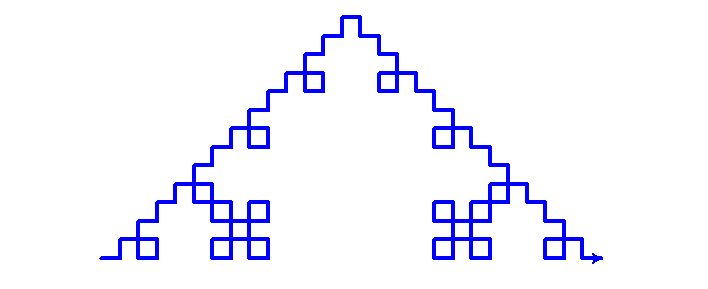
\includegraphics[scale=0.22]{ecran-lsysteme-3c}
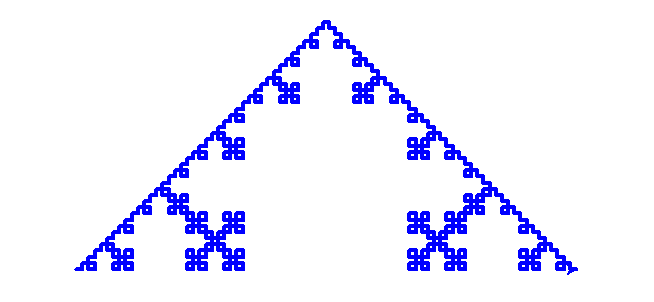
\includegraphics[scale=0.22]{ecran-lsysteme-3d}
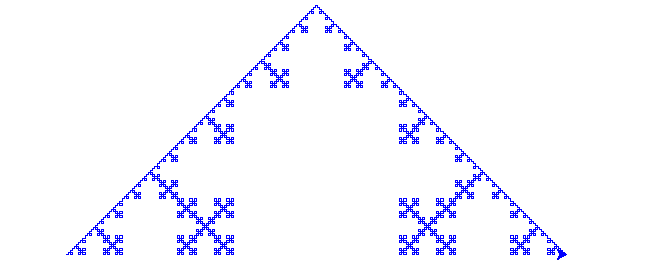
\includegraphics[scale=0.22]{ecran-lsysteme-3e}
\end{center}
  
	\item Trace d'autres figures fractales à partir des L-systèmes suivants. Pour tous ces exemples le mot de départ est \ci{"AdAdAdA"} (un carré) et la règle est à choisir parmi :
	
\medskip	
		
	\begin{itemize}
	  \item \ci{("A"," AdAgAgAAdAdAgA")}
	  \item \ci{("A","AgAAdAAdAdAgAgAAdAdAgAgAAgAAdA")}
	  \item \ci{("A","AAdAdAdAdAA")}
	  \item \ci{("A","AAdAddAdA")}
	  \item	\ci{("A","AAdAdAdAdAdAgA")}
	  \item \ci{("A","AAdAgAdAdAA")}
	  \item \ci{("A","AdAAddAdA")}
	  \item \ci{("A","AdAgAdAdA")}
	\end{itemize}
	
\medskip	
	
\begin{center}
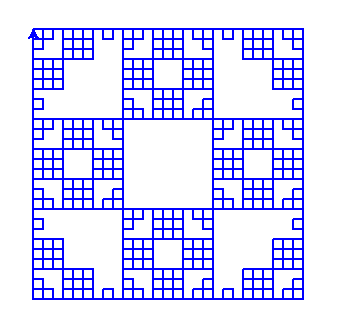
\includegraphics[scale=0.3]{ecran-lsysteme-4}\quad
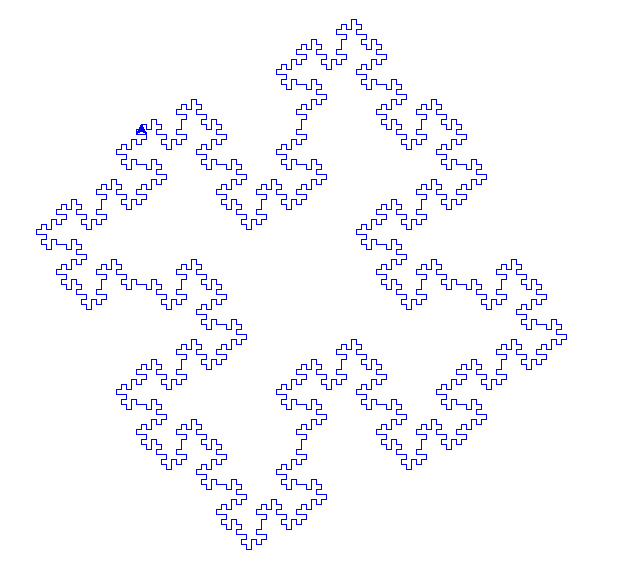
\includegraphics[scale=0.2]{ecran-lsysteme-5}\quad
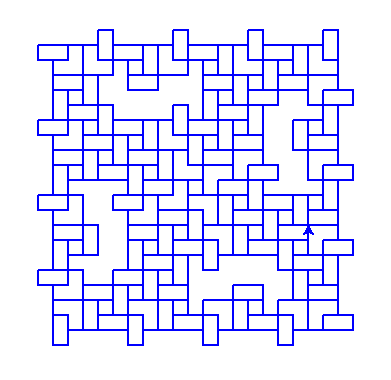
\includegraphics[scale=0.27]{ecran-lsysteme-6}
\end{center}


\end{enumerate}


\objectifs{Invente et trace tes propres L-systèmes !}

\end{activite}



%%%%%%%%%%%%%%%%%%%%%%%%%%%%%%%%%%%%%%%%%%%%%%%%%%%%%%%%%%%%%%%%
% Activité 3
%%%%%%%%%%%%%%%%%%%%%%%%%%%%%%%%%%%%%%%%%%%%%%%%%%%%%%%%%%%%%%%%

\begin{activite}[Deux règles -- Triangle de Sierpinski]

\objectifs{Objectifs : calculer des L-systèmes plus compliqués en autorisant cette fois deux règles de remplacement au lieu d'une seule.}

\index{triangle de Sierpinski}

\begin{center}	
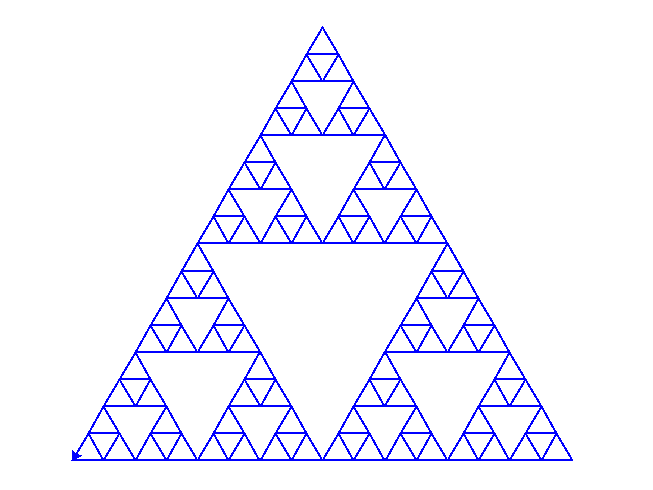
\includegraphics[scale=0.35]{ecran-lsysteme-7e}
\end{center}

\begin{enumerate}
  \item Programme une fonction \ci{remplacer_2(mot,lettre1,motif1,lettre2,motif2)} qui remplace une première lettre par un motif et une seconde lettre par un autre. 

Par exemple avec \ci{mot = "AdBgA"}, \ci{remplacer_2(mot,"A","ABg","B","Bd")} renvoie le mot \ci{ABgdBdgABg} : chaque lettre \mot{A} a été remplacée par le motif \mot{ABg} et en même temps chaque lettre \mot{B} a été remplacée par le \mot{Bd}.

\emph{Attention !} Il ne faut pas obtenir \ci{ABdgdBdgABdg}. Si c'est le cas c'est que tu as utilisé la fonction \ci{remplacer_1()} pour d'abord remplacer les \ci{A}, puis une seconde fois pour les \ci{B} (mais après le premier remplacement de nouveaux \ci{B} sont apparus). Il faut reprogrammer une nouvelle fonction pour éviter cela. 

 
  \item Programme une fonction \ci{iterer_lsysteme_2(depart,regle1,regle2,k)}
  qui calcule le $k$-ème itéré du L-système associé au mot initial \ci{depart} selon les règles \ci{regle1} et \ci{regle2}.
   Par exemple, avec :
  \begin{itemize} 
    \item \ci{depart = "AdBdB"}
    \item \ci{regle1 = ("A","AdBgAgBdA")} c'est-à-dire \mot{A} $\rightarrow$ \mot{AdBgAgBdA}
    \item \ci{regle2 = ("B","BB")} c'est-à-dire \mot{B} $\rightarrow$ \mot{BB}  
    \item pour \ci{k = 0}, la fonction renvoie le mot de départ \ci{AdBdB},
    \item pour \ci{k = 1}, la fonction renvoie \ci{AdBgAgBdAdBBdBB},
    \item pour \ci{k = 2}, la fonction renvoie :\\ 
    \centerline{\ci{AdBgAgBdAdBBgAdBgAgBdAgBBdAdBgAgBdAdBBBBdBBBB}}
  \end{itemize}  

  \item Trace les premières images du triangle de Sierpinski donné comme ci-dessus par : \\
  \centerline{départ : \mot{AdBdB} \qquad règles : \mot{A} $\rightarrow$ \mot{AdBgAgBdA} \quad \mot{B} $\rightarrow$ \mot{BB}} 
 L'angle est de $-120$ degrés. Voici les images pour $k=0$ jusqu'à $k=4$.
  
\begin{center}
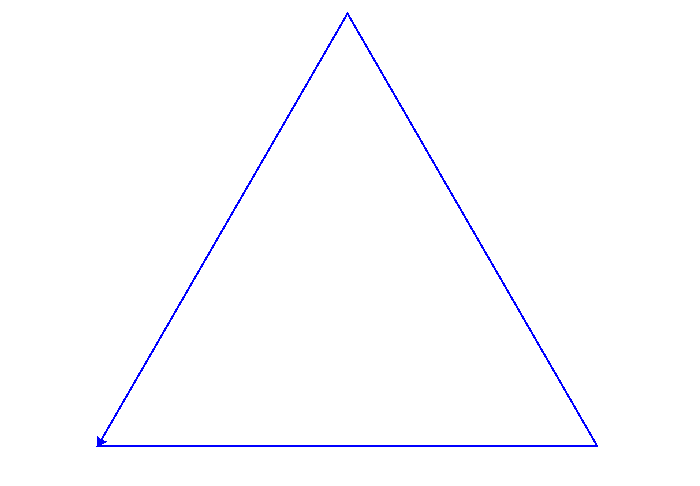
\includegraphics[scale=0.22]{ecran-lsysteme-7a}
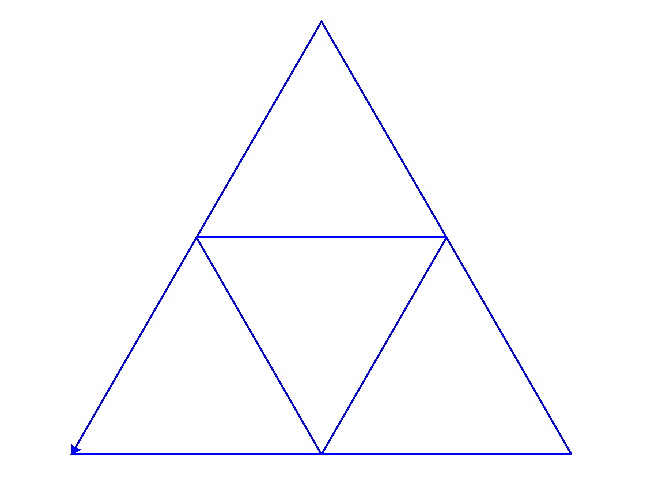
\includegraphics[scale=0.22]{ecran-lsysteme-7b}
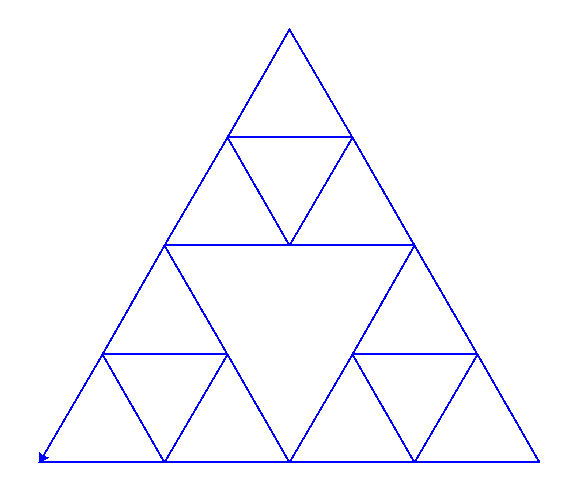
\includegraphics[scale=0.22]{ecran-lsysteme-7c}
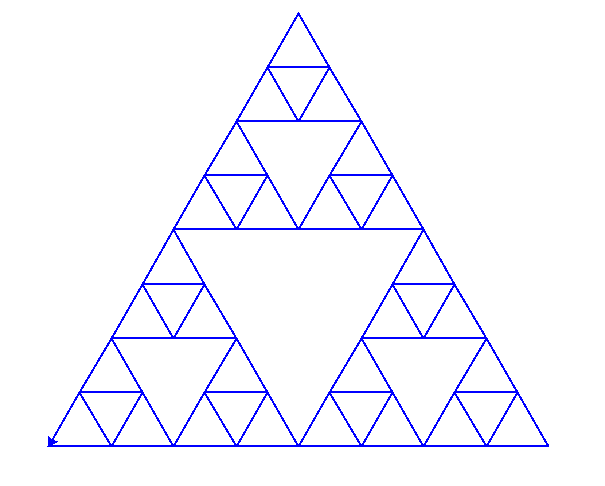
\includegraphics[scale=0.22]{ecran-lsysteme-7d}
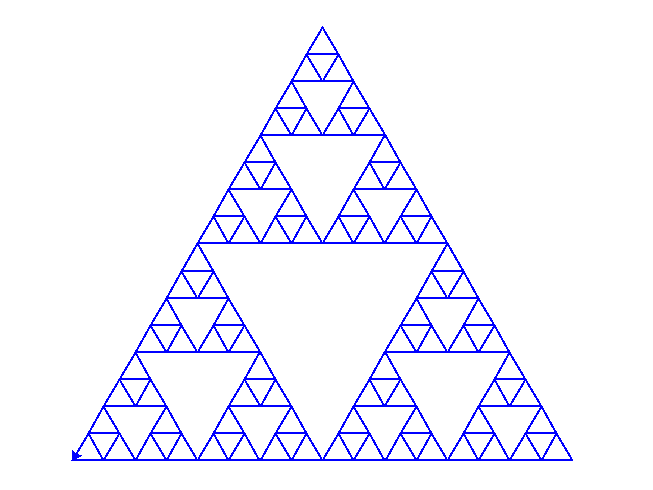
\includegraphics[scale=0.22]{ecran-lsysteme-7e}
\end{center}
  
	\item Trace d'autres figures fractales à partir des L-systèmes suivants.
	
	\begin{itemize}
	  \item La courbe du dragon :\\
\centerline{\ci{
depart="AX"    
regle1=("X","XgYAg")    
regle2=("Y","dAXdY")
}}

Les lettres \ci{X} et \ci{Y} ne correspondent à aucune action.

	\item Une variante du triangle de Sierpinski, avec \ci{angle = 60} :\\
\centerline{\ci{	
depart="A"    
regle1=("A","BdAdB")    
regle2=("B","AgBgA")
}}

\item La courbe de Gosper, avec \ci{angle = 60} :\\	 
\centerline{\ci{ 
depart="A"    
regle1=("A","AgBggBdAddAAdBg")    
regle2=("B","dAgBBggBgAddAdB")
}}
	  
	\end{itemize}
	
\begin{center}
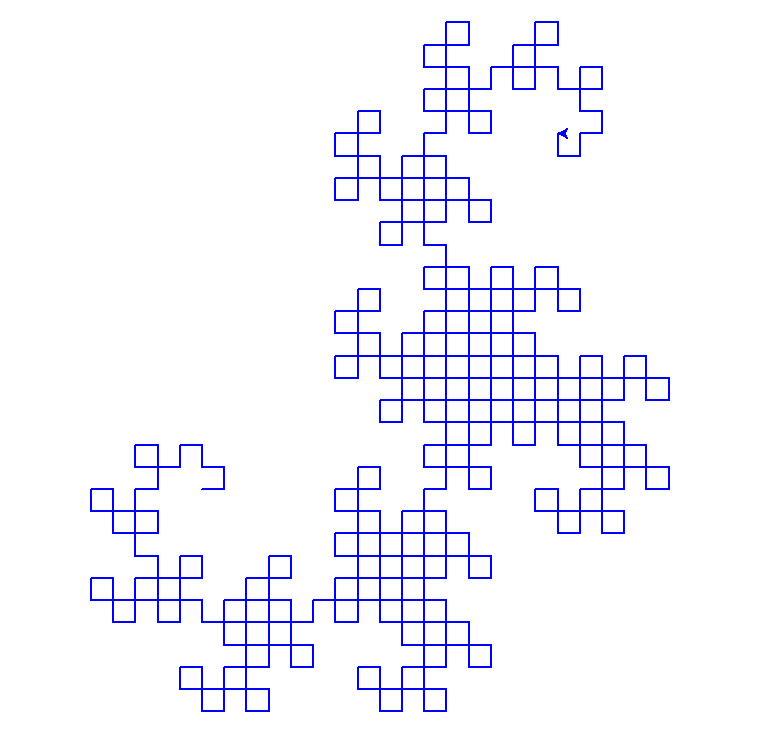
\includegraphics[scale=0.15]{ecran-lsysteme-8}\quad
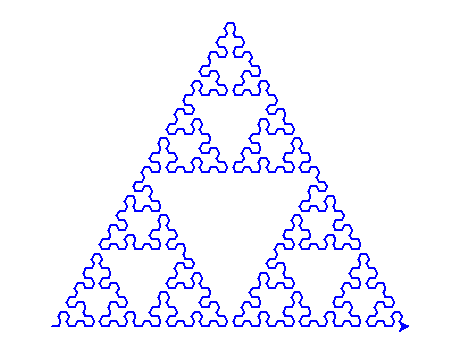
\includegraphics[scale=0.33]{ecran-lsysteme-9}\quad
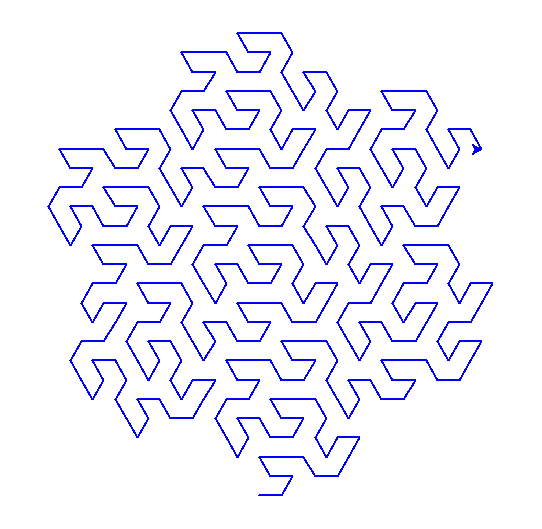
\includegraphics[scale=0.24]{ecran-lsysteme-10}
\end{center}


\end{enumerate}

\objectifs{Invente et trace tes propres L-systèmes avec deux règles !}


\end{activite}


\begin{cours}[Piles]
Une \defi{pile} est une zone de stockage temporaire. Les détails sont dans la fiche \og{}Calculatrice polonaise -- Piles\fg{}. Voici juste quelques rappels.

\index{pile}

\myfigure{1}{
\tikzinput{fig-piles}
}  

\begin{itemize}
  \item Une pile c'est comme un pile d'assiettes ; on pose des éléments un par un au-dessus de la pile ; on retire les éléments un par un, également à partir du dessus. C'est le principe : \og{}dernier arrivé, premier parti\fg{} (\emph{last in, first out}).
  
  \item On modélise une pile par une liste. 
  \item Au départ la pile est vide : \ci{pile = []}.
  \item \textbf{Empiler.} On ajoute les éléments en fin de liste : \ci{pile = pile + [element]}.
  \item \textbf{Dépiler.} On retire un élément par la commande \ci{pop()}\index{pop@\ci{pop}}\index{depiler@dépiler} :\\
  \centerline{\ci{element = pile.pop()}}
  qui renvoie le dernier élément de la pile et le supprime de la liste.
  
  \item Sur le dessin et dans l'activité suivante, les éléments de la pile sont du type $\big((x,y),\theta\big)$  qui stockeront un état de la tortue : $(x,y)$ est la position et $\theta$ sa direction.
  
\end{itemize}

\end{cours}


%%%%%%%%%%%%%%%%%%%%%%%%%%%%%%%%%%%%%%%%%%%%%%%%%%%%%%%%%%%%%%%%
% Activité 4
%%%%%%%%%%%%%%%%%%%%%%%%%%%%%%%%%%%%%%%%%%%%%%%%%%%%%%%%%%%%%%%%

\begin{activite}[L-système et tortue à pile]

\objectifs{Objectifs : améliorer nos tracés en autorisant d'avancer sans tracer et aussi à l'aide d'une sorte de retour en arrière, afin de tracer des plantes.}

\begin{center}
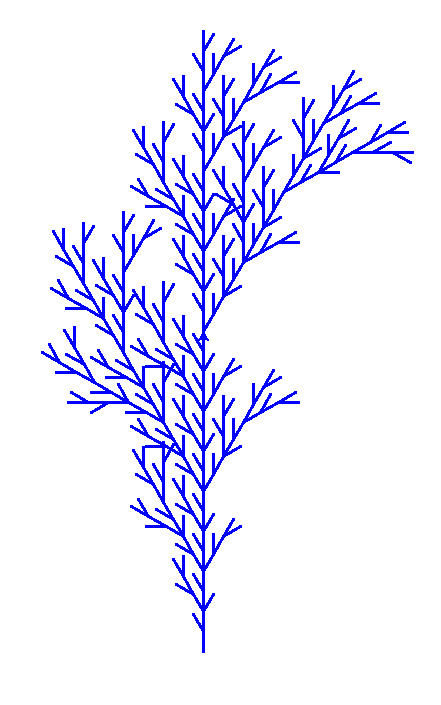
\includegraphics[scale=0.25]{ecran-lsysteme-17}
\end{center}

\begin{enumerate}
  \item \textbf{Avancer sans tracer.} 
  
  Augmente les possibilités en autorisant la tortue à avancer sans tracer de trait, lorsque l'instruction est la lettre est \mot{a} (en minuscule). (Il suffit de modifier la
fonction \ci{trace_lsysteme()}.)

Trace alors le L-système suivant :
\begin{itemize}  
\item \ci{depart = "AdAdAdA"}
\item \ci{regle1 = ("A","AgadAAgAgAAgAagAAdagAAdAdAAdAadAAA")}
\item \ci{regle2 = ("a","aaaaaa")}
\end{itemize}
\begin{center}
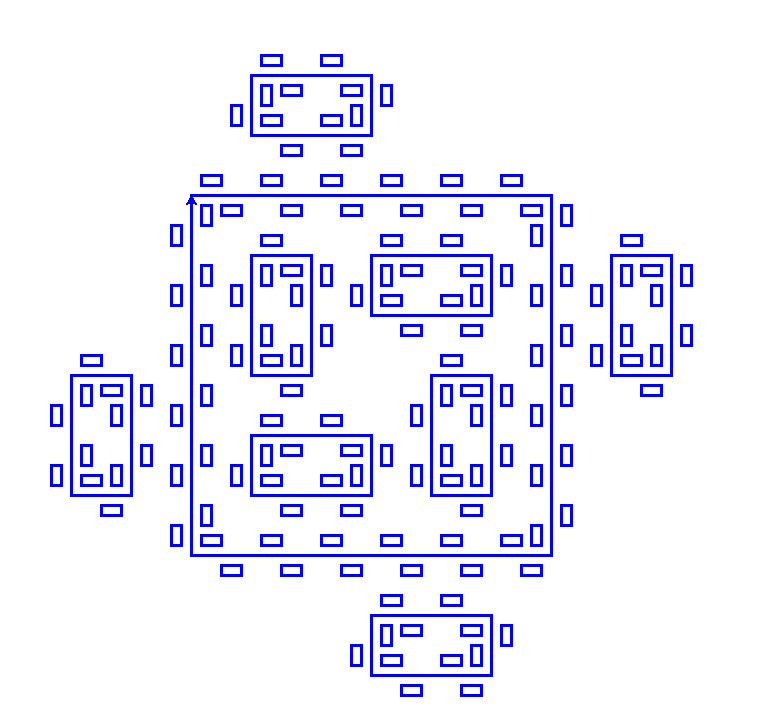
\includegraphics[scale=0.2]{ecran-lsysteme-11}
\end{center}  

  \item \textbf{Retour en arrière.} 
  
  On autorise maintenant des crochets dans nos mots. Par exemple \mot{AgA[gAAA]A[dAA]A}. Lorsque l'on rencontre un crochet ouvrant \og{}\mot{[}\fg{}, on mémorise la position de la tortue, puis les commandes entre crochets sont exécutées comme d'habitude, lorsque l'on trouve un crochet fermant \og{}\ci{]}\fg{} on repart de la position mémorisée auparavant.
  
  
Comprenons l'exemple du tracé du 
\mot{
{\color{blue}AgA}
{\color{red}[gAAA]}
{\color{green!70!black}A}
{\color{purple}[dAA]}
{\color{orange}A}
}. 
\myfigure{1}{
\tikzinput{fig-crochets}
}    
\begin{itemize}
  \item \mot{{\color{blue}AgA}} : on part du point $O$, on avance, on tourne, on avance.
  \item \mot{{\color{red}[gAAA]}} : on retient la position actuelle (le point $P$) et aussi la direction ; on tourne, on avance trois fois (on trace le segment rouge) ; à la fin on replace la tortue à la position $P$ (sans tracer et avec la même direction que celle auparavant).
  \item \mot{{\color{green!70!black}A}} : depuis $P$ on avance (segment vert).
  \item \mot{{\color{purple}[dAA]}} : on retient la position $Q$ et la direction, on tourne et on trace le segment violet. On revient en $Q$ avec l'ancienne direction.
  \item \mot{{\color{orange}A}} : depuis $Q$ on trace le dernier segment.
\end{itemize}

  \medskip
  
  Voici comment tracer un mot contenant des crochets à l'aide d'une pile :
  \begin{itemize}
    \item Au départ la pile est vide.
	\item On lit un par un les caractères du mot. Les actions sont les mêmes qu'auparavant.
	\item Si le caractère est le crochet ouvrant \og{}\mot{[}\fg{} alors on ajoute à la pile la position et la direction courante de la tortue $\big( (x,y), \theta\big)$ que l'on obtient par \ci{(position(), heading())}.
	
	\item Si le caractère est le crochet fermant \og{}\mot{]}\fg{} alors dépiler 
	(c'est-à-dire lire l'élément du haut de la pile et le retirer). Mettre la position de la tortue et l'angle avec les valeurs lues, utiliser \ci{goto()} et \ci{setheading()}.
	
	\end{itemize}
	
	\item Trace les L-systèmes suivants, où l'on donne le mot de départ et la règle (ou les règles). L'angle est à choisir entre $20$ et $30$ degrés.
	
\begin{itemize}

	  \item 
\ci{"A"}
\ci{("A","A[gA]A[dA][A]")}
	  
	  \item 
\ci{"A"}
\ci{("A","A[gA]A[dA]A")}
	  
	  \item 
\ci{"A"}
\ci{("A","AAd[dAgAgA]g[gAdAdA]")}

	  \item 
\ci{"X"} 
\ci{("X","A[gX][X]A[gX]dAX")} 
\ci{("A","AA")}
	  
	\item 
\ci{"X"}
\ci{("X","A[gX]A[dX]AX")}
\ci{("A","AA")}

	\item 
\ci{"X"}
\ci{("X","Ad[[X]gX]gA[gAX]dX")}
\ci{("A","AA")}
	\end{itemize}
	
\begin{center}
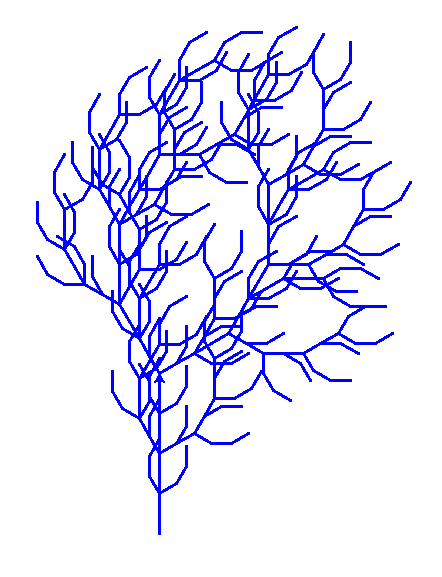
\includegraphics[scale=0.27]{ecran-lsysteme-15}\qquad
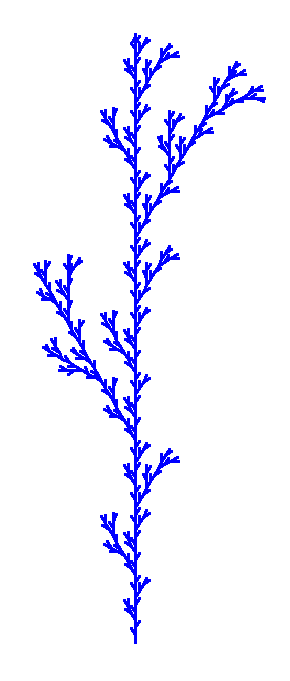
\includegraphics[scale=0.25]{ecran-lsysteme-16}\qquad
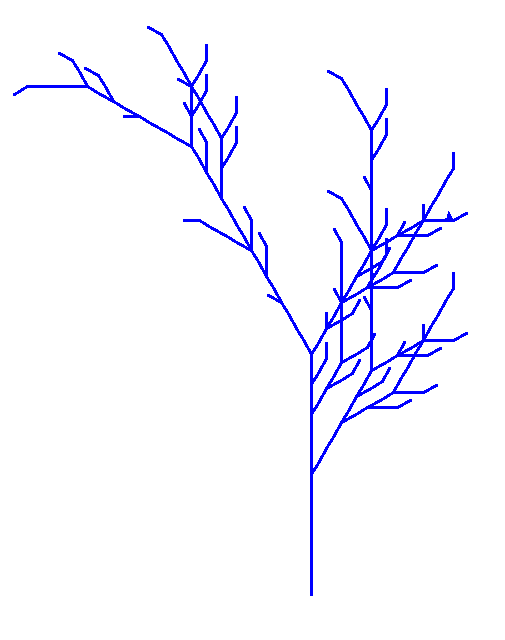
\includegraphics[scale=0.25]{ecran-lsysteme-12}
\end{center}
	
  
 \end{enumerate}

\objectifs{Invente ta propre plante !}

\end{activite}

\end{document}
